\documentclass[11pt]{exam}

\usepackage{amsmath, amssymb, multicol}
\usepackage{graphicx}
\usepackage{textcomp}
\usepackage{chessboard}

\def\d{\displaystyle}
\def\b{\mathbf}
\def\R{\mathbf{R}}
\def\Z{\mathbf{Z}}
\def\st{~:~}
\def\bar{\overline}
\def\inv{^{-1}}

\def\v{circle (3pt)}


%\pointname{pts}
\pointsinmargin
\marginpointname{pts}
\addpoints
\pagestyle{head}
%\printanswers

\firstpageheader{Math 228}{\bf From Dots to Sequences}{Wednesday, October 24}


\begin{document}

%space for name
%\noindent {\large\bf Name:} \underline{\hspace{2.5in}}
%\vskip 1em

\subsection*{Activity 1: Dots}

For the patterns of dots below, draw the next pattern in the sequence.  Then give a recursive definition and a closed formula for the number of dots in the $n$th pattern.


  \begin{multicols}{4}

\vspace*{\fill}


    \begin{center}

  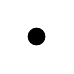
\begin{tikzpicture}
  \draw[fill = black] (0,0) \v;
  \end{tikzpicture}

  $n = 0$
  \end{center}


  \columnbreak
\vspace*{\fill}


    \begin{center}
    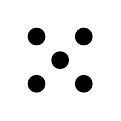
\begin{tikzpicture}
    \draw[fill = black] (0,0) \v (.3, .3) \v (-.3,-.3) \v (-.3, .3) \v (.3,-.3) \v;
    \end{tikzpicture}

    $n = 1$
    \end{center}

    \columnbreak
    \vspace*{\fill}

    \begin{center}
    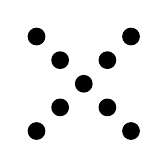
\begin{tikzpicture}
    \draw[fill = black] (0,0) \v (.3, .3) \v (-.3,-.3) \v (-.3, .3) \v (.3,-.3) \v (.6, .6) \v (-.6,-.6) \v (-.6, .6) \v (.6,-.6) \v;
    \end{tikzpicture}

    $n = 2$
    \end{center}

    \columnbreak
\vspace*{\fill}
	~
  \end{multicols}


  \begin{solution}
  The next pattern will contain 13 dots.  Since each pattern will contain 4 more dots than the previous, the recursive definition will be $a_n = a_{n-1} + 4$; $a_0 = 1$.  The closed formula will be $a_n = 1 + 4n$.
  \end{solution}

\vfill




  \begin{multicols}{4}

  \vspace*{\fill}
  \begin{center}
  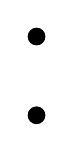
\begin{tikzpicture}
  \draw[fill = black] (0,0) \v (0,1) \v;
  \end{tikzpicture}

  $n = 0$
  \end{center}

  \columnbreak

  \vspace*{\fill}
    \begin{center}
    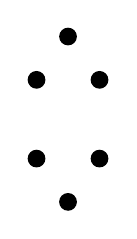
\begin{tikzpicture}
    \draw[fill = black] (-.4,0) \v (.4, 0) \v (0, -.55) \v (-.4,1) \v (.4, 1) \v (0,1.55) \v;
    \end{tikzpicture}

    $n = 1$
    \end{center}

    \columnbreak

    \vspace*{\fill}
    \begin{center}
    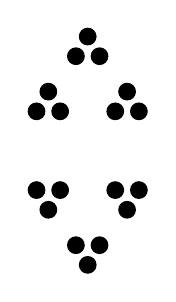
\begin{tikzpicture}
    \draw[fill = black] (-.65,0) \v (-.35,0) \v (-.5,-.25) \v
    	(.35, 0) \v (.65,0) \v (.5, -.25) \v
    	(-.15, -.7) \v (.15, -.7) \v (0, -.95) \v
    	(-.65, 1) \v (-.35, 1) \v (-.5,1.25) \v
    	(.35, 1) \v (.65, 1) \v (.5, 1.25) \v
    	(-.15,1.7) \v (.15, 1.7) \v (0,1.95) \v;
    \end{tikzpicture}

    $n = 2$
    \end{center}

    \columnbreak

   \vspace*{\fill}

    ~
  \end{multicols}

\begin{solution}
The next figure will have 54 dots.  Each figure is created by splitting each dot into 3, so each will be 3 times the previous.  This leads directly to the recursive definition: $a_n = 3a_{n-1}$; $a_0 = 2$.   The closed formula is $a_n = 2\cdot 3^n$.
\end{solution}



\vfill
%Triangular Numbers.
  \begin{multicols}{5}

  \vspace*{\fill}
  \begin{center}
  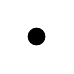
\begin{tikzpicture}
  \draw[fill = black] (0,0) \v;
  \end{tikzpicture}

  $n = 1$
  \end{center}

  \columnbreak

  \vspace*{\fill}
    \begin{center}
    
\begin{tikzpicture}
    \draw[fill = black] (0,0) \v (.5, 0) \v (.25,.4) \v;
    \end{tikzpicture}

    $n = 2$
    \end{center}

    \columnbreak

    \vspace*{\fill}
    \begin{center}
    
\begin{tikzpicture}
    \draw[fill = black] (0,0) \v (.5, 0) \v (.25,.4) \v (1,0) \v (.75,.4) \v (.5, .8) \v;
    \end{tikzpicture}

    $n = 3$
    \end{center}

    \columnbreak

    \vspace*{\fill}
        \begin{center}
        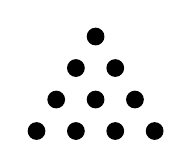
\begin{tikzpicture}
        \draw[fill = black] (0,0) \v (.5, 0) \v (.25,.4) \v (1,0) \v (.75,.4) \v (.5, .8) \v (1.5, 0) \v (1.25, .4) \v (1, .8) \v (.75, 1.2) \v;
        \end{tikzpicture}

        $n = 4$
        \end{center}

        \columnbreak
     \vspace*{\fill}
     ~
  \end{multicols}

 \begin{solution}
 The next patter will contain 15 dots.  These are the triangular numbers.  Each one is found by adding a new row of dots (one longer than the previous row).  Thus $a_n = a_{n-1} + n$; $a_1 = 1$ is the recursive definition.  A closed formula is $a_n = \frac{n(n+1)}{2}$.

 \end{solution}
\vfill

\newpage

\subsection*{Activity 2: Sequences}

For each sequence of numbers, guess the next term in  the sequence.  Then find a recursive definition and closed formula for the $n$th term of the sequence.  Assume the first term given is $a_0$.

\begin{itemize}
\item 3, 6, 12, 24, \ldots
\begin{solution}
Recursive: $a_n = 2a_{n-1}$; $a_0 = 3$.  Closed: $a_n = 3 \cdot 2^n$.
\end{solution}
\vfill
\item 2, 5, 8, 11, \ldots
\begin{solution}
Recursive: $a_n = a_{n-1} + 3$; $a_0 = 2$.  Closed: $a_n = 2 + 3n$.
\end{solution}
\vfill
\item 4, 12, 20, 28, \ldots
\begin{solution}
Recursive: $a_n = a_{n-1} + 8$; $a_0 = 4$.  Closed: $a_n = 4 + 8n$.
\end{solution}
\vfill
\item 4, 12, 36, 108, \ldots
\begin{solution}
Recursive: $a_n = 3a_{n-1}$; $a_0 = 4$.  Closed: $a_n = 4\cdot 3^n$.
\end{solution}
\vfill
\item 2, 5, 10, 17, 26, \ldots
\begin{solution}
Recursive: $a_n = a_{n-1} + 2n+1$; $a_0 = 2$.  Closed: $a_n = (n+1)^2 + 1$ (if you notice that each is one more than a perfect square) or $a_n = \frac{2+(2n+4)n}{2}$ (which is the same, but is what you get if you notice this is the sum of an arithmetic sequence).
\end{solution}
\vfill
\item $1, 5, 17, 53, 161,\ldots$
\begin{solution}
  Recursive: $a_n = a_{n-1} + 4\cdot 3^{n-1}$; $a_0 = 1$.  To find a closed formula we must find the sum of the geometric sequence $4, 12, 36, 108,\ldots$.  We would get $a_n =2\cdot 3^n - 1$ (where the $-1$ is really $1 + -2$; the $1$ comes from the $a_0$).
\end{solution}
\end{itemize}



\end{document}
